\documentclass[a4paper,12pt]{report}
\usepackage{graphicx} % Include the graphicx package for images
\usepackage{geometry} % Include geometry package for adjusting page size
\usepackage{fancyhdr} % Include fancyhdr package for headers and footers
\usepackage{lipsum} % Include lipsum package for placeholder text (optional)


\newgeometry{left=0in,right=0in,top=0in,bottom=0in}
    \begin{titlepage}
        \begin{center}
            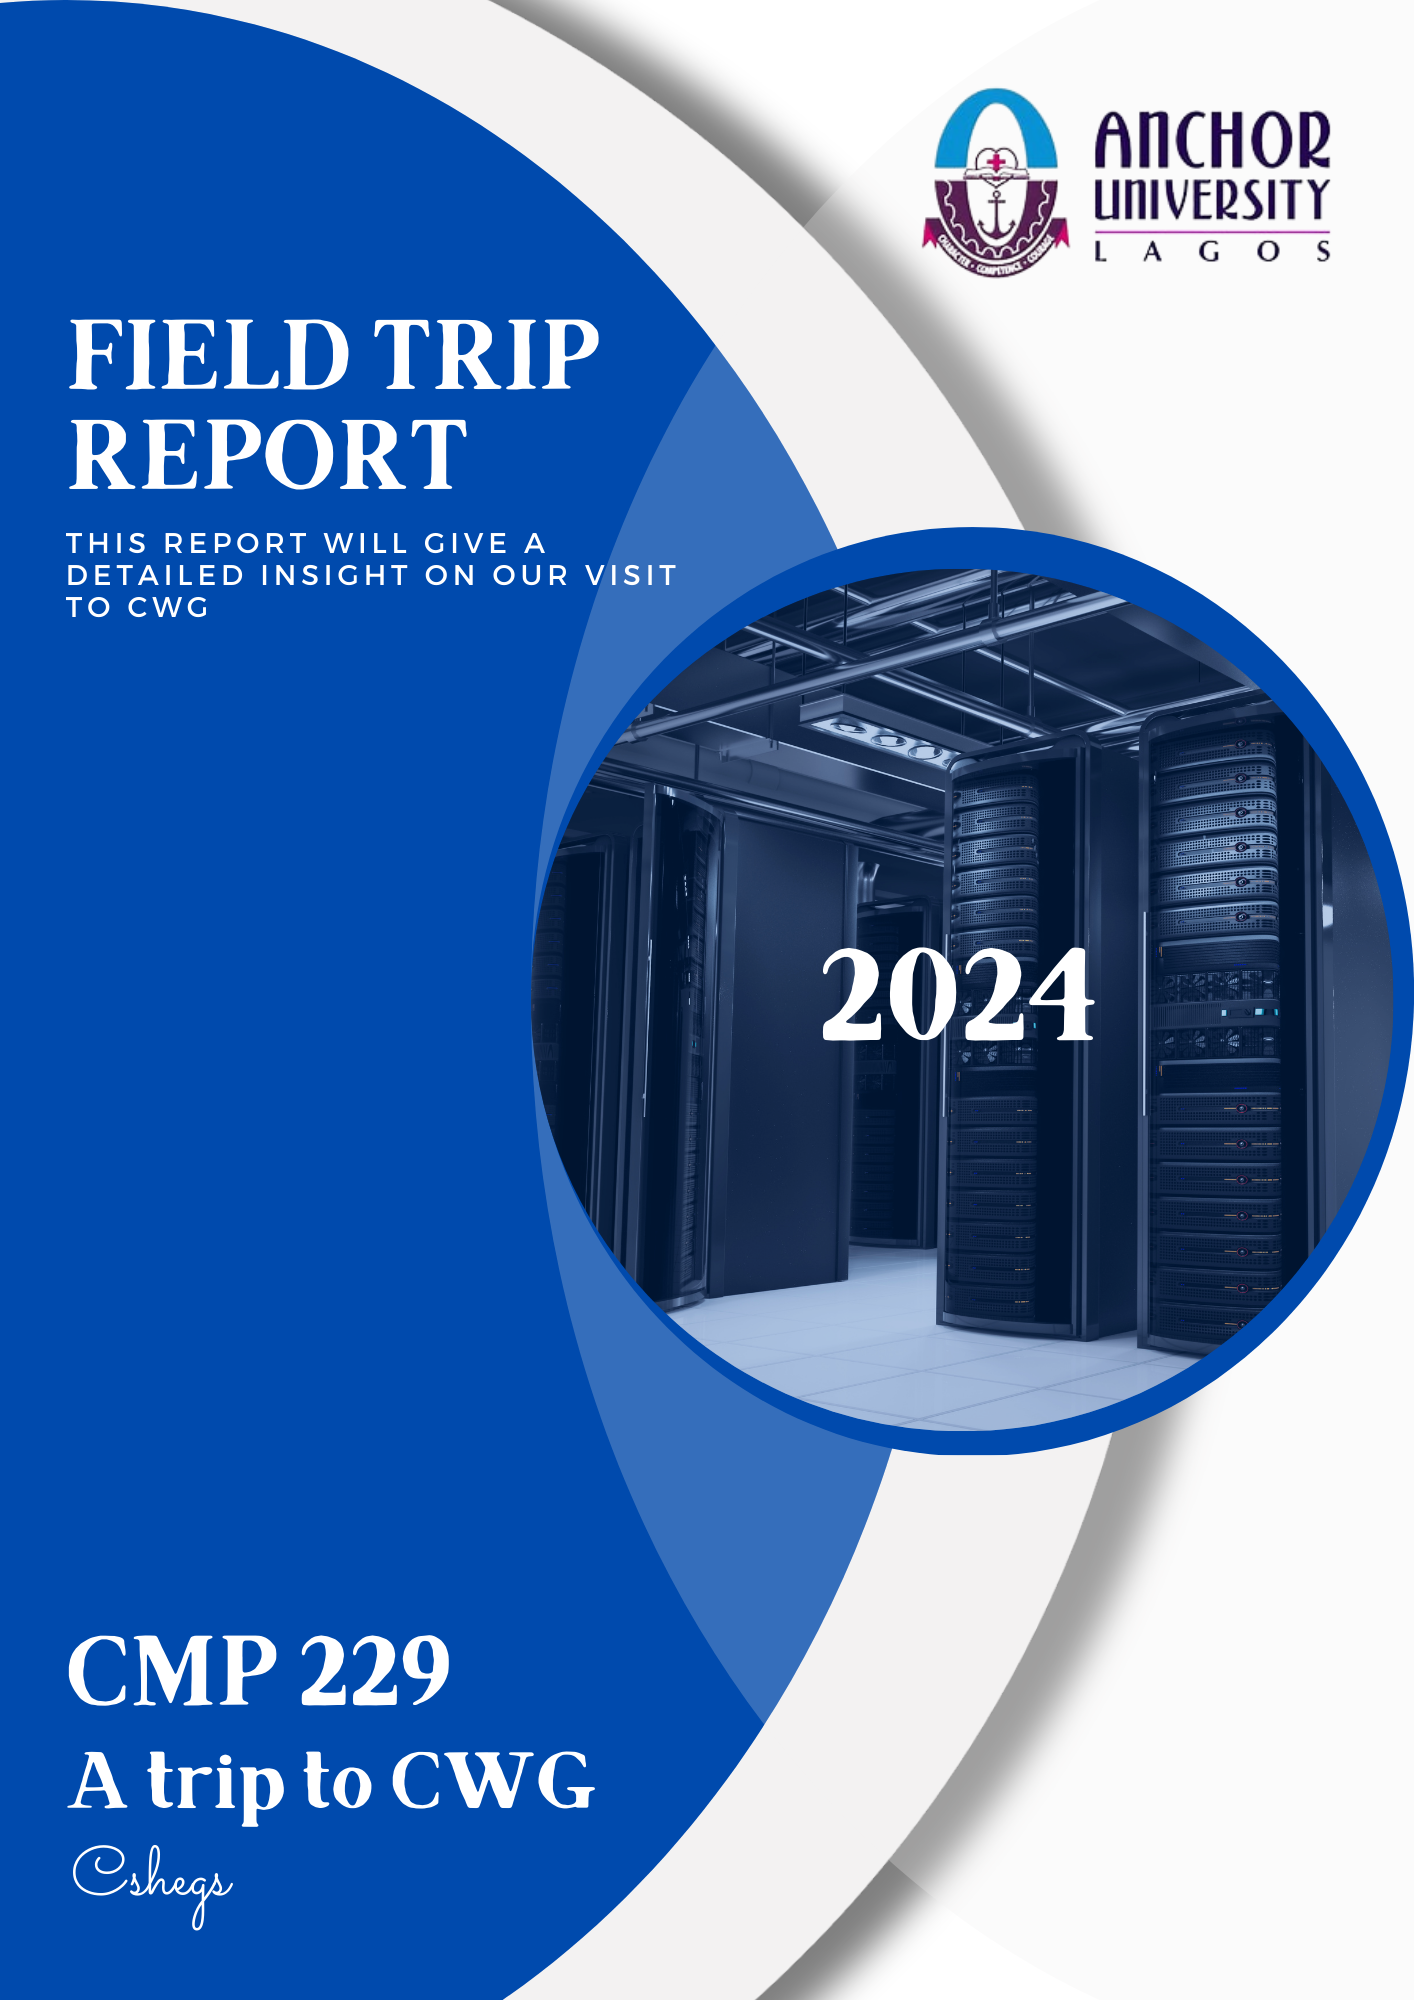
\includegraphics[width=\paperwidth, height=\paperheight]{Field trip cover photo.png}
    \end{center}
\end{titlepage}
\restoregeometry

\title{A FIELD TRIP REPORT ON THE VISIT TO CWG PLC BY ANCHOR UNIVERSITY LAGOS COMPUTER SCIENCE STUDENTS}
\author{Agboola Oluwasegun \\
        AUL/CMP/22/011 \\
        COMPUTING DEPARTMENT \\
        CMP 229 REPORT \\
        FIELD TRIP}
\date{Thursday 13th June, 2024}

\begin{document}

\maketitle

\tableofcontents

\pagenumbering{roman}

\begin{abstract}
    This report provides a comprehensive account of a field trip undertaken by Anchor University Lagos, 200 level undergraduate computer science students to CWG Plc, a leading provider of information and communication technology solutions in Africa. The primary objective of the field trip was to bridge the gap between academic learning and practical industry experience.

During the visit, students were exposed to various operational facets of CWG, including their data centers, cloud services, and software development processes. The trip included guided tours, technical demonstrations, and interactive sessions with CWG professionals, who shared insights into current industry trends and challenges. Pre-trip preparation involved research and goal setting, while post-trip activities included reflective essays and presentations to reinforce learning outcomes.

The field trip to CWG significantly enhanced the students' understanding of real-world applications of computer science principles. It provided a practical perspective on topics such as network security, data management, and software engineering, which are critical components of their academic curriculum. The experience also fostered greater enthusiasm and motivation among students to pursue careers in the technology sector.

In conclusion, the field trip to CWG was a valuable educational experience that effectively complemented the theoretical knowledge gained in the classroom. It underscored the importance of hands-on learning and industry engagement in shaping the future careers of computer science students.
\end{abstract}

\pagenumbering{arabic}

\chapter[Chapter 1]{INTRODUCTION}
One this day, Wednesday 29th May, 2024, I and about 50 other colleagues of Anchor University Lagos, 200 Level, Computing Department went on a paid field trip to the Prestigious Computer Wear-house Group (CWG). It was a very resourceful and insightful trip as we were introduced to the practical-real-world reality of the IT world.

\section[Definition]{DEFINITION OF FIELD TRIP}
Field trips, also known as educational excursions, are visits to locations outside the regular classroom environment, aimed at providing students with practical experiences and opportunities to apply theoretical knowledge in real-world settings. For undergraduate students, particularly in computer science, field trips play a crucial role in bridging the gap between academic learning and industry practices.

\section[Importance]{IMPORTANCE OF FIELD TRIP}
\begin{enumerate}
    \item \textbf{Hands-On Experience:} Field trips allow students to see and interact with technologies and processes they learn about in class. This hands-on experience is invaluable in solidifying their understanding and enhancing their practical skills.
    \item \textbf{Industry Exposure:} Visits to tech companies, data centers, or research labs expose students to the latest advancements in the field, giving them a glimpse into potential career paths and emerging trends.
    \item \textbf{Networking Opportunities:} These trips provide a platform for students to meet and network with professionals in the industry, which can be beneficial for future internships and job opportunities.
    \item \textbf{Stimulate Interest and Motivation:} o inspire students by showcasing cutting-edge technologies and innovative solutions, motivating them to pursue further studies or careers in specific areas of interest.
\end{enumerate}

\section[Objectives]{OBJECTIVES OF FIELD TRIPS AS A COURSE}
Field The primary objectives of the field trip to CWG Plc were multifaceted and aimed at enhancing the educational experience of the 200-level computer science students at Anchor University Lagos. The objectives were designed to bridge the gap between theoretical knowledge and practical industry applications. They included:

\begin{enumerate}
    \item \textbf{Enhance Practical Knowledge:} To provide students with direct exposure to the tools, techniques, and workflows used in the industry.
    \item \textbf{Foster Critical Thinking:} To encourage students to analyze and understand the complexities of real-world problems and how they are addressed by professionals.
    \item \textbf{Promote Teamwork and Collaboration:} To develop teamwork skills as students often work in groups during field trips, fostering collaboration and communication skills.
    \item \textbf{Stimulate Interest and Motivation:} To inspire students by showcasing cutting-edge technologies and innovative solutions, motivating them to pursue further studies or careers in specific areas of interest.
\end{enumerate}

\section[Study mode]{MODE OF STUDY}
The mode of study for the field trip was structured to maximize learning outcomes through a combination of pre-trip preparation, on-site activities, and post-trip reflection. They include:
\subsection{Pre-Trip Preparation:} This involves background research on the destination, setting learning goals, and understanding the expectations. Instructors may provide reading materials or assignments to prepare students.    
    \begin{itemize}
        \item \textbf{Research:} Prior to the visit, students conducted research on CWG Plc, understanding its history, mission, and the services it provides. This was to ensure that students were well-informed and could engage meaningfully during the trip.
        \item \textbf{Goal Setting:} Students were required to set personal learning goals for the trip. These goals were aligned with the objectives of the field trip and tailored to each student’s interests and academic needs.
    \end{itemize}
    
\subsection{On-Site Activities:} 
    \begin{itemize}
        \item \textbf{Guided Tours:} The visit included guided tours of CWG’s data centers, cloud services, and software development facilities. These tours were led by experienced professionals who explained the workings of each department.
        \item \textbf{Technical Demonstrations:} Students attended technical demonstrations where they observed the practical application of various technologies. These demonstrations covered topics such as network security, data management, and software engineering.
        \item \textbf{Interactive Sessions:} Interactive sessions were held with CWG professionals. During these sessions, students had the opportunity to ask questions, discuss industry trends, and learn about the challenges faced in the ICT sector.
    \end{itemize}

\subsection{Post-Trip Activities:}
    \begin{itemize}
        \item \textbf{Report Writing:} After the trip, students were required to write report on their experiences. These helped to consolidate their learning and provided an opportunity to reflect on how the visit enhanced their understanding of computer science principles.
        \item \textbf{Presentations:} Students also prepared presentations to share their experiences, learning outcomes with their peers and to submit it on the provided Google Classroom Environment. This activity promoted collaborative learning and allowed students to articulate their insights and knowledge gained from the trip.
    \end{itemize}


The structured approach to the field trip ensured that students not only gained practical knowledge but also developed a deeper understanding of the real-world applications of their academic studies, thereby complementing their theoretical education with valuable industry exposure.

\chapter[Chapter 2]{ORGANIZATION}
\section[History]{HISTORY OF CWG}
CWG Plc, formerly known as CMB Wireless Group, was founded in 1992 by Austin Okere. It has grown to become a leading provider of information and communication technology solutions in Africa. The company was initially established to provide hardware sales and support services but has since expanded its offerings to include a broad range of ICT services.
The current CEO of Communication Wireless Group, LLC (CWG) is Adewale Adeyipo. He has been in this role since 2018, first as Acting MD/CEO and later confirmed.

\section[Motto]{MOTTO OF CWG}
CWG’s motto is "Championing the New Africa," reflecting its commitment to driving technological innovation across the continent.

\section[Mission]{MISSION OF CWG}
The mission of CWG is to enable businesses and organizations across Africa to achieve more by providing reliable and cutting-edge IT solutions.

\section[Vision]{VISION OF CWG}
CWG envisions being the leading IT solutions provider in Africa, fostering growth and development through technology.

\section[Core values]{CORE VALUES}
\begin{itemize}
    \item \textbf{Excellence:} Committed to delivering high-quality services.
    \item \textbf{Innovation:} Continuously improving and introducing new solutions.
    \item \textbf{Integrity:} Maintaining transparency and honesty in all dealings.
    \item \textbf{Customer Focus:} Prioritizing customer needs and satisfaction.
\end{itemize}

\section[partners]{PARTNERSHIPS:} CWG has established numerous partnerships with global technology leaders to enhance its service offerings and provide comprehensive solutions. These partnerships include collaborations with major IT firms and local enterprises to foster technological advancement in Africa. Some of her partners are listed below;
\begin{itemize}
    \item Infosys
    \item AMEYO
    \item MICROSOFT
    \item HITACHI
    \item IBM
    \item VERITAS
    \item CISCO
    \item NUTANIX
    \item NEWGEN
    \item RED HAT
    \item NETAPP
    \item DELL - EMC
\end{itemize}

\section[Branches]{BRANCHES}
CWG operates presently across 5 countries, namely Nigeria, Ghana, Uganda, Cameroon, and UAE (United Arab Emirates). Each branch is strategically positioned to serve regional markets effectively.

\section[Sections]{SECTIONS}
CWG’s operations are divided into various sections, each specializing in different IT services such as:
\begin{itemize}
    \item \textbf{Brand and Marketing Department:} Handles design and their public image. 
    \item \textbf{Sales Department:} Push out their work to the outer world.
    \item \textbf{Customer Support:} Help customers develop and have quality experience with their product.
    \item \textbf{Quality Assurance (QA):} Ensure they meet standard values.
    \item \textbf{Human Resources:} Take care of the work-force (workers). They organize from time-to-time, conferences, Forum, Seminar, Etc.. for her workers.
    \item \textbf{information technology (IT):} Resposible for keeping her technology infrastructure running smoothly.
    \item \textbf{Software Development:} Skilled developers take ideas generated by the R and D team and turn them into reality.
    \item \textbf{Date Center:} Responsible for managing her data storage and processing needs. It houses the server and other hardware that store and process the amount of data to be reliable.
\end{itemize}

\chapter[Chapter 3]{DISCUSSION}
We were walked into the CWG room on the wall which wrote "WELCOME TO CWG". Memu Moses, Head of the ICT was the first to give his presentation. He started by asking Five (5) of us to introduce ourselves and state our career path. In his presentation it was stated that "CWG is a qualified information and communication technology company. We're not your ordinary company; we're a team of passionate individuals who love to think outside the box and push the boundaries of what's possible. Whether it's developing cutting-edge software or designing user-friendly apps, we're always striving to make a positive impact on the real world. Our company was founded with the belief that technology can be a powerful tool for innovation and progress."

\paragraph{}
As at the time of our visit, they were celeberating 32 years of industry experience

\paragraph{}
The IT head also stated that "they provided about $94,724,265$ bank customers support, they are behind daily transaction cost of about $182,500,000$, supporting about 11.6 Million daily ATM transactions and get about 40 Million number of transactions"

\section[Awards]{AWARDS}

\paragraph{list of some of her awards are below}
\begin{itemize}
    \item \textbf{Award by NTA:} Software as a service provider of the year 2022.
    \item \textbf{Award by Nigeria Communications Week:} E-Commerce Platform of the year, 2015.
    \item \textbf{Award by NiTA:} CWG wins Technology Support Company of the Year 2019.
    \item \textbf{Award by Fidelity Bank:} Distinguished SME Partner Award, 2014, Austin Okere.
    \item \textbf{Award by CISCO:} DCC wins Cisco Gold Certified Partner in West Africa, 2013.
\end{itemize}
and many more others Etc...

\section[Fifth lab]{FIFTH LAB}
Mrs Akintola, Business director of CWG and Fifth lab was welcomed in to tell us about it.
Fifth Lab is a fintech app which first major launch was in 2022. It's was the application designed for the fintech unit of CWG.

\subsection[Fifth lab Mission]{MISSION OF FIFTH LAB}
The mission is to create simplified solutions that makes life and work easy

\subsection[Fifth lab Vision]{VISION OF FIFTH LAB}
To build high tech IT solutions that empower people and businesses

\subsection[PDLC]{PRODUCT DEVELOPMENT LIFE CYCLE}
We were taught about 5 Product development life cycle which principle was reponsible behind the functioning of Fifth lab and they are;
\begin{enumerate}
    \item \textbf{Ideation: }This is the initial phase where you come up with the idea for your project. It's the brainstorming stage where you define the concept and identify the problem your product aims to solve. You outline the goals and scope of the project, considering feasibility and potential impact.
    \item \textbf{Product Design: }In this phase, the initial idea is translated into a blueprint for development. This includes creating wireframes, user interface (UI) designs, and defining the user experience (UX). Detailed specifications are documented to guide the development team. This stage ensures that the product will be user-friendly and meet the needs of the target audience.
    \item \textbf{Product Development: }Here, the actual coding begins. Front-end developers work on the client side of the application, focusing on aspects like layout, design, and interactivity. Back-end developers handle server-side logic, database interactions, and integration of various components. Collaboration between front-end and back-end teams is crucial to build a functional product.
    \item \textbf{Testing Phase: }During this stage, the product undergoes rigorous testing to identify and fix any bugs or issues. You get people around you, including potential users and quality assurance (QA) testers, to test the product. The mission is to ensure the product is stable, secure, and performs as expected. Feedback from testers is used to make necessary adjustments and improvements.
    \item \textbf{Product Launch: }Once testing is complete and the product is polished, it's ready for launch. This involves deploying the product to the market, whether through app stores, websites, or other distribution channels. A launch plan is executed, including marketing and promotional activities to ensure the product reaches its intended audience and gains traction.
\end{enumerate}

\subsection[Product CATALOG]{FIFTH LAB PRODUCT CATALOG}
\begin{enumerate}
    \item \textbf{Finedge:} Core banking application, is a financial planning and advisory firm that offers personalized financial solutions. The firm provides services such as investment planning, wealth management, and financial goal-setting. 
    \item \textbf{Kulean pay:} Escrow platform, used to solve the problem around scams or a "What I ordered vs what I got situation". A simple analogy to define how the Kuleanpay program works is, I pay Kuleanpay then when the vendor deliverd it, we can tell Kuleanpay to approve transfer. This kind of system would bring about transparency to business transactions going on everyday. 
    \item \textbf{Billsnpay VAS:} Manages Airtime vending platform 
    \item \textbf{Smerp/SmerpGO:} SMERP which stands for small medium enterprise resource planning platform was designed to handle businesses for people by performing invoicing management, account management Etc.
          \paragraph{SmerpGo} This is the solution designed to make running of your business easy, allowing you take picture of your business. It was created for micro and nano organizations.  
    \item \textbf{UCP:} Unified Communication Platform refers to an integrated system that consolidates various communication tools and channels into a single platform. It aims to streamline communication, increase productivity, and improve overall organizational efficiency.
    \item \textbf{Gaming:} Helps government gets proper records consigning tax funds from gaming platforms in the country such as casinos, online betting platforms Etc..
\end{enumerate}

\section[IT]{INFORMATION TECHNOLOGY}
We were told on the need to study Information Technology
\begin{enumerate}
    \item It's skills are sought after the industry and is crying out for talents.
    \item It has a growing job marketing.
    \item You will never be bored, career and intellectual growth are guaranteed.
    \item Ability to work for your dream company (in any Country)
\end{enumerate}

\subsection[IT careers]{CAREERS IN IT}
\begin{itemize}
    \item web developement
    \item Game Development
    \item System analyst
    \item System engineer
    \item Network administrator
    \item Database administrator
\end{itemize}

\section[SQL]{STRUCTURED QUERY LANGUAGE}
Daniel Odigbo, senior software developer at CWG took us through this section. SQL which stands for structured query language is used for building core banking applications. A example is Finacle which is a core app used by 80 percent banks in Nigeria for their application.
\paragraph{}
SQL is the only language database understands but they have limitations as they can't accomodate performimg multiple level transactions at the same time, and that's where PLSQL comes in play as you can fetch data and do multiple transaction (insert, delete, read) at the same time.

\section[Infrastructure]{INFRASTRUCTURE}
This houses all other sections, it's necessary to have one. The Infrastructure Head reminded us that "AI will replace only those that don't know how to use AI". He brought this to our notice when he explained how hee as a supivisor does his duty by assigning some mini tasks to the AI. 

\section[Human resource]{HUMAN RESOURCE}
The final presentation was done by Mrs. Tinuade, the head of HR department. Where she spoke about work ethics in the work space. Few things she spoke about are;
\begin{itemize}
    \item \textbf{Attitude:} Your attitude in the workplace can significantly impact your career. A positive attitude fosters a cooperative and productive work environment. It can help you build strong relationships with colleagues, handle challenges with resilience, and maintain motivation. A proactive, can-do attitude is often noticed by supervisors and can lead to career advancement opportunities.
    \item \textbf{Respect:} Respect in the workplace involves recognizing the value of others, regardless of their position, background, or opinions. It means listening actively, valuing diverse perspectives, and treating everyone with courtesy. Respectful behavior helps build a positive work culture, reduces conflicts, and promotes collaboration. It also contributes to a sense of belonging and morale among team members.
    \item \textbf{Value:} Value in a professional context refers to both the value you bring to your organization and the value you place on your work and colleagues. Bringing value means delivering quality work, being reliable, and contributing to the team's goals. It also involves recognizing the contributions of others and acknowledging their efforts. Demonstrating your value consistently can lead to greater job satisfaction, recognition, and career growth.
    \item \textbf{Self Development:} Self-development is the continuous process of improving your skills, knowledge, and personal qualities. In the workplace, this could mean seeking out training opportunities, learning new technologies, or developing soft skills like communication and leadership. Investing in self-development shows a commitment to your career and can make you more adaptable and valuable to your employer. It also positions you for advancement and helps you stay competitive in your field.
\end{itemize}
\paragraph{}
She also added that "You have to be extra to be extraordinary"

\section[Tour]{TOUR}
The presentation section lead to the tour section where we visited six (6) sections of the company. The first was fifth lab where the set up was for software development as alligning to their aim during it's creation in 2022. The second place was the "Dish Receptor which was used to transmit and receive data and signals". The third place was the Power house where we saw different back up measures to keep power supply intact because of the data-base operations. The forth place, "Network operation center". The fifth place, "Data center", and finally "The metering unit". I would explain the function of the centers we visited below.

\subsection[Satalite communication]{SATALITE TRANSMISSION SYSTEM}
\begin{itemize}
    \item \textbf{The Dish Receptor:} A dish receptor, commonly known as a satellite dish, is a type of parabolic antenna designed to receive or transmit information from a satellite. The primary function of the dish is to focus the incoming satellite signals onto the feed horn. The parabolic shape of the dish allows it to collect signals from a large area and concentrate them into a single point, enhancing the signal strength.
    \item \textbf{Low Noise Block (LNB):} The Low Noise Block (LNB) is a critical component mounted on the feed horn of a satellite dish. Its primary function is to amplify the weak satellite signals collected by the dish and convert them to a lower frequency band for easier processing. The term "low noise" refers to the LNB's ability to amplify signals without adding much noise, which is crucial for maintaining signal quality.
    \item \textbf{High Power Amplifier (HPA):} A High Power Amplifier (HPA) is used in satellite communication systems to boost the power of the signal before it is transmitted to the satellite. This amplification is necessary to ensure that the signal can travel the long distance to the satellite without significant loss of strength. HPAs are typically used in the uplink part of the communication system.
\end{itemize}

\paragraph{}
During our tour in CWG, these components played a significant role in demonstrating the process of satellite communication. The dish receptor collects the satellite signals, the LNB amplifies and converts these signals for further processing, and the HPA boosts the signal power for transmission. Understanding these components and their functions provides a comprehensive view of how satellite communication systems operate.

\subsection[Power house]{POWER HOUSE}
During our tour of the power house at CWG, we learned about their backup power supply system. The key components included the Automatic Transfer Switch \textbf{(ATS)} and several named machines: \textbf{PHCN}, \textbf{Castle 1}, and \textbf{Castle 2}. The system is designed to ensure uninterrupted power to the database.

\paragraph{Here’s how it works:}
\begin{itemize}
    \item \textbf{PHCN} is the primary power source. When \textbf{PHCN} fails, the ATS automatically switches the power control to \textbf{Castle 1}.
    \item If \textbf{Castle 1} is also unavailable, the ATS transfers control to \textbf{Castle 2}.
\end{itemize}

\paragraph{}
To further ensure a constant power supply, CWG has two industrial generators as additional backups. The instructor emphasized the importance of maintaining continuous power in the database, with no downtime allowed.
The system includes several other components:
\begin{itemize}
    \item \textbf{Voltage Regulator:} Maintains voltage between 220V and 230V to prevent damage.
    \item \textbf{Contactor:} Manages high and low voltage situations.
    \item \textbf{Heavy Duty Stabilizers:} Used for the cooling system in the data center to ensure stable operation.
    \item \textbf{Phase Control Panel (PCP):} Contains various components including a timer switch and in-rack ATS modules, each with a capacity of 20 KVA.
\end{itemize}

\paragraph{}
One critical observation was the significant expense associated with maintaining such a comprehensive power backup system.

\subsection[Network center]{NETWORK OPERATION CENTER}
\paragraph{}
During our tour of the Network Operations Center (NOC) at CWG, we had the opportunity to interact with the network operation center engineers who explained how they monitor and manage the network. They provide network services to several top channels, including TVC, ensuring that traffic is efficiently directed to these channels. Additionally, they offer video services to these clients.

\paragraph{}
In the NOC, I observed practical applications of concepts we learned in our Network Fundamentals course (CMP 223). The engineers demonstrated real-time network monitoring, traffic management, and troubleshooting techniques. It was fascinating to see how theoretical concepts such as network protocols, bandwidth management, and network security are applied in a real-world setting to maintain seamless network operations.

\paragraph{}
Overall, the visit provided a valuable insight into the practical aspects of network management and reinforced the importance of the concepts we studied in CMP 223.

\subsection[Data center]{DATA CENTER}
During our visit to the data center at CWG, we observed multiple servers housed in structures known as racks, each serving various clients. Each rack contains several servers, ensuring organized and efficient management of resources.

\paragraph{}
The data center is equipped with two HVAC (Heating, Ventilation, and Air Conditioning) units to regulate temperature and ensure proper cooling of the servers. Additionally, the facility uses FM-200 gas for fire suppression. This gas is crucial for safety as it works by displacing oxygen to extinguish fires without damaging the equipment.

\paragraph{}
We also noted the presence of a proximity sensor and a well-marked emergency exit, both essential for safety in case of a fire. The servers, being components of computer circuits, can overheat and pose a fire risk, making these safety measures vital.

\paragraph{}
The data center is maintained with a proper cooling system and is kept clean regularly to prevent dust and debris accumulation, which could affect the equipment. The emphasis on safety and maintenance practices was evident throughout our visit.

\subsection[Metering unit]{METERING UNIT}
During our visit to the metering unit at CWG, we learned about their role as a manufacturing and meter acceptance provider. They focus on the production and provision of prepaid meters, which record and measure energy consumption over time.

\paragraph{}
One key aspect of their operation is the test bench, where they rigorously test the meters for accuracy to ensure they conform to industry standards. This process is critical for maintaining reliability and precision in energy measurement.

\paragraph{}
The visit provided valuable insights into how these meters are produced, tested, and validated, highlighting the importance of accurate energy consumption measurement in the industry.

\chapter[Summary, Conclusion, Recommendation]{SUMMARY, CONCLUSION, AND RECOMENDATION}

\section[Summary]{SUMMARY}
During our tour of CWG, we visited several key areas that provided us with a comprehensive understanding of the technical operations and infrastructure necessary for a successful IT environment. We explored Fifthlab, the Power House, the Network Operations Center, the Data Center, and the Metering Unit.

\begin{itemize}
    \item \textbf{Power House:} We learned about the critical components ensuring uninterrupted power supply, including the Automatic Transfer Switch (ATS), various backup systems (PHCN, Castle 1, Castle 2), industrial generators, voltage regulators, heavy-duty stabilizers, and Phase Control Panels (PCP).
    \item \textbf{Network Operations Center (NOC):} We observed how network operation center engineers monitor and manage networks, ensuring efficient traffic flow and providing video services to top channels. This visit demonstrated practical applications of network management concepts from our coursework.
    \item \textbf{Data Center:} We saw multiple servers housed in racks, supported by advanced HVAC systems for cooling and FM-200 gas for fire suppression. Safety measures, such as proximity sensors and emergency exits, were in place to prevent and manage potential fire hazards.
    \item \textbf{Metering Unit:} This unit manufactures and tests prepaid meters for accuracy, ensuring they meet industry standards. We learned about the importance of accurate energy consumption measurement and the rigorous testing process involved.
\end{itemize}

\section[Conclusion]{CONCLUSION}
The visit to CWG was highly beneficial, providing us with practical insights into various IT operations and infrastructure management. We gained a deeper understanding of how theoretical concepts are applied in real-world settings, particularly in power management, network operations, data center management, and metering accuracy. This hands-on experience has reinforced our classroom learning and highlighted the importance of maintaining robust and reliable IT systems.

\section[Recommendation]{RECOMMENDATION}
To further enhance the benefits of such visits, we recommend the following:
\begin{itemize}
    \item \textbf{Regular Industry Tours:} Organize regular tours to different IT facilities to expose students to various aspects of the industry.
    \item \textbf{Hands-On Workshops:} Arrange workshops where students can engage in practical tasks related to power management, network monitoring, and data center operations.
    \item \textbf{Guest Lectures:} Invite industry professionals to give talks on current trends and challenges in IT infrastructure and management.
    \item \textbf{Internship Opportunities:} Facilitate internships with companies like CWG to provide students with real-world experience and professional networking opportunities.
\end{itemize}

\section[Career Enhancement]{CAREER ENHANCEMENT}
The knowledge and experience gained from this trip are invaluable for our future careers in IT. Understanding the intricacies of power supply management, network operations, data center infrastructure, and metering systems will make us more adept at handling real-world challenges. This exposure not only enhances our technical skills but also gives us a competitive edge in the job market, paving the way for successful careers in IT infrastructure and management.

\chapter[References]{REFERENCES}
\begin{itemize}
    \item \textit{Kolb, D. A. (1984). Experiential Learning: Experience as the Source of Learning and Development. Prentice-Hall.
    \item CWG Plc. (n.d.). About Us. Retrieved from CWG Plc Official Website.
    \item Lam, A. (2010). Bridging the Gap Between Theory and Practice in Computer Science Education. ACM SIGCSE Bulletin, 42(3), 33-37.
    \item D. A. (1983). The Reflective Practitioner: How Professionals Think in Action. Basic Books.}
\end{itemize}

\end{document}
